\chapter{A unifying logic for the Semantic Web} \label{uni}

%why especially the last feature mentioned, the proof format, makes it a good 
%option to be the unifying logic for the Semantic Web.





% In order to enable the computer to read from the Web, understand it and draw its own conclusions different technologies are needed: first of all, knowledge needs to be 
% represented in an unambiguous way. It is rather difficult for the computer to decide whether the term \emph{bass} refers to a fish or a musical instrument, 
% but by using different 
% unique names employing Uniform Resource Identifiers (\uris) it can clearly distinguish between  \texttt{dbr:Bass_guitar}.

% When humans process language, a lot of knowledge is required. To decide whether the term \emph{bass} refers to a fish or a musical instrument they need context.
% If humans browse through the Web, they read written content which they are able to process because of their knowledge of the world. Without 

% All of us have already tried to directly talk to the computer---especially when we were frustrated and nothing seemed to work---but even when we scream in such situations, 
% the computer's reaction is rather disappointing. A lot of afford is made to change this situation and to enable the computer to understand natural language, 
% but there are still obstacles: human language tends to be ambiguous. Without knowing the context it is hard to tell whether the term 

% In order to ``teach'' the computer these concepts, it needs to be able to parse the language used and to make sense of it. 
% And even though there is an agreement that this language cannot be natural language---with all its ambiguities which are impossible or at least very difficult to resolve by a 
% machine---but that a logic is needed, the opinions about the nature of that logic differ: description logic based formalisms are very powerful and allow for complex reasoning but they 
% are also sensible for mistakes.



\section{The vision of the Semantic Web}
My idea for this chapter is to explain a little bit more about the semantic web in general and its architecture


\section{Architecture}

Gerber \cite{Gerber} \cite{Gerber2}. Really nice: abstracts from technnologies. Bad: the word ``unifying Logic'' dissapeared.

\cite{rearch} Paper by Boley, Kifer, etc. ``realistic'' architecture, not just one technology. 

\begin{figure}[h!]
	\centering
	%\begin{adjustwidth}{-\marginnotewidth}{}%
	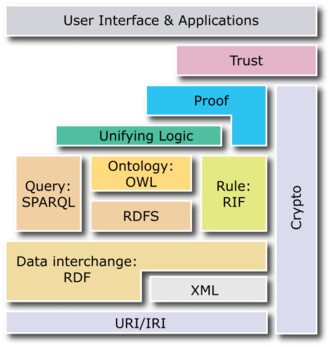
\includegraphics{Semantic_Web_Stack}
	%\end{adjustwidth}
	\caption{Semantic Web Stack. Source: \url{https://www.w3.org/2007/03/layerCake.svg}}
	\label{fig:stack}
\end{figure}
\subsection{Data Interchange}
RDF

\cite{rdf}
\subsection{Querying}
\subsection{Ontologies}
RDFS
OWL
\subsection{Rule Based Logics}
RIF

SWRL

N3

\cite{N3Logic}

\subsection{Unifying Logic}
What do we expect from the ``unifying logic''?

The vision of the Semantic Web is to enable machines to use the Web just as humans do. For that they need to be able to \emph{understand} and \emph{exchange} data through the Web. 
An unambiguous way to express knowledge is needed, a logic. 
This logic needs to be well defined to avoid misunderstandings and it needs to be agreed on this definition between all possible parties involved.


Also say why you should go for N3: unifying logic is not just a theoretical construct, it also gives practical advantages: reasoning is often faster when you use only one logic.  
It has advantages if you need 
the features of different frameworks. Of course, if you know that, eg only querying is needed you should still go for SPARQL.


% The Unifying Logic needs to be well-defined in itself, it needs to be able to ``understand'' the underlying formats, in particular to query, do DL reasoning and use rules. 
% Additionally it should provide the opportunity to connect to the proof layer.
Requirements:
\begin{description}
 \item[clear semantic definition] 
The meaning of every statement needs to be clearly defined.
 \item[compatibility with existing Web standards]  Existing standards of the Semantic Web need to be supported. 
 In particular, querying, Description Logics, and rule based reasoning need to be covered.
 \item[support of proofs] It must be possible to express, interchange and check all derivations made in the logic.
 \item[capability to handle change] It must be possible to express and reason about change.
\end{description}
\subsection{Proofs}
\section{Research questions}
Question: Is N3 a suitable candidate to become the unifying logic for the semantic web?

Sub-questions:

Can we give a clear semantic definition of Notation3 Logic?

How does Notation3 Logic interfere with other formats? Can SPARQL, OWL and RIF be expressed?

Is it possible to express proofs in N3?

Can N3 handle change?

I think I need to be more specific. To find that: what do I actually do here?



% \textbf{Part 4: going beyond the limits}
% 
% introduce weighted transition logic to express change
% 
% This part is optional



Somewhere I need to talk about problems, especially decidability and for example the problems of OWL full.